\documentclass[aspectratio=169]{beamer}
\usepackage[T1]{fontenc}
\usepackage{lmodern}
\usepackage[utf8]{inputenc}
\usepackage[polish]{babel}
\usepackage{amsmath,graphicx}
\usetheme{Madrid}
\usecolortheme{seahorse}
\title{Oscylator harmoniczny}
\subtitle{Od prawa Hooke'a do rezonansu}
\author{Przykładowa prezentacja}
\date{\today}
\begin{document}

\begin{frame}
  \titlepage
\end{frame}

\begin{frame}
  \frametitle{Plan}
  \tableofcontents
\end{frame}

\section{Model}
\begin{frame}
  \frametitle{Układ masa--sprężyna}
  \begin{itemize}
    \item Masa $m$ porusza się wzdłuż jednej osi.
    \item Sprężyna o sztywności $k$ działa siłą $F_s=-kx$.
    \item $x=0$ oznacza położenie równowagi.
  \end{itemize}
  \begin{block}{Założenie modelu}
    Pomijamy masę sprężyny i opory ruchu.
  \end{block}
\end{frame}

\begin{frame}
  \frametitle{Równanie ruchu}
  Z drugiej zasady Newtona:
  \begin{equation*}
    m\ddot x=-kx,\qquad
    \ddot x+\omega_0^2x=0,\qquad
    \omega_0=\sqrt{\frac{k}{m}}.
  \end{equation*}
  \begin{exampleblock}{Kontrola wymiarów}
    $[k/m]=\mathrm{s}^{-2}$, więc $[\omega_0]=\mathrm{s}^{-1}$.
  \end{exampleblock}
\end{frame}

\section{Rozwiązanie}
\begin{frame}
  \frametitle{Rozwiązanie z warunkami początkowymi}
  Dla $x(0)=x_0$ i $\dot x(0)=v_0$:
  \begin{equation*}
    x(t)=x_0\cos(\omega_0t)+
    \frac{v_0}{\omega_0}\sin(\omega_0t).
  \end{equation*}
  \begin{enumerate}
    \item Wyznacz $\omega_0$ z $m$ i $k$.
    \item Wstaw warunki początkowe.
    \item Sprawdź, czy pochodna w $t=0$ daje $v_0$.
  \end{enumerate}
\end{frame}

\begin{frame}
  \frametitle{Energia oscylatora}
  \begin{columns}[T]
    \begin{column}{.44\textwidth}
      \begin{block}{Energia kinetyczna}
        $E_k=\tfrac12m\dot x^2$
      \end{block}
      \begin{block}{Energia potencjalna}
        $E_p=\tfrac12kx^2$
      \end{block}
      $E=E_k+E_p=\tfrac12kA^2$ jest stała.
    \end{column}
    \begin{column}{.53\textwidth}
      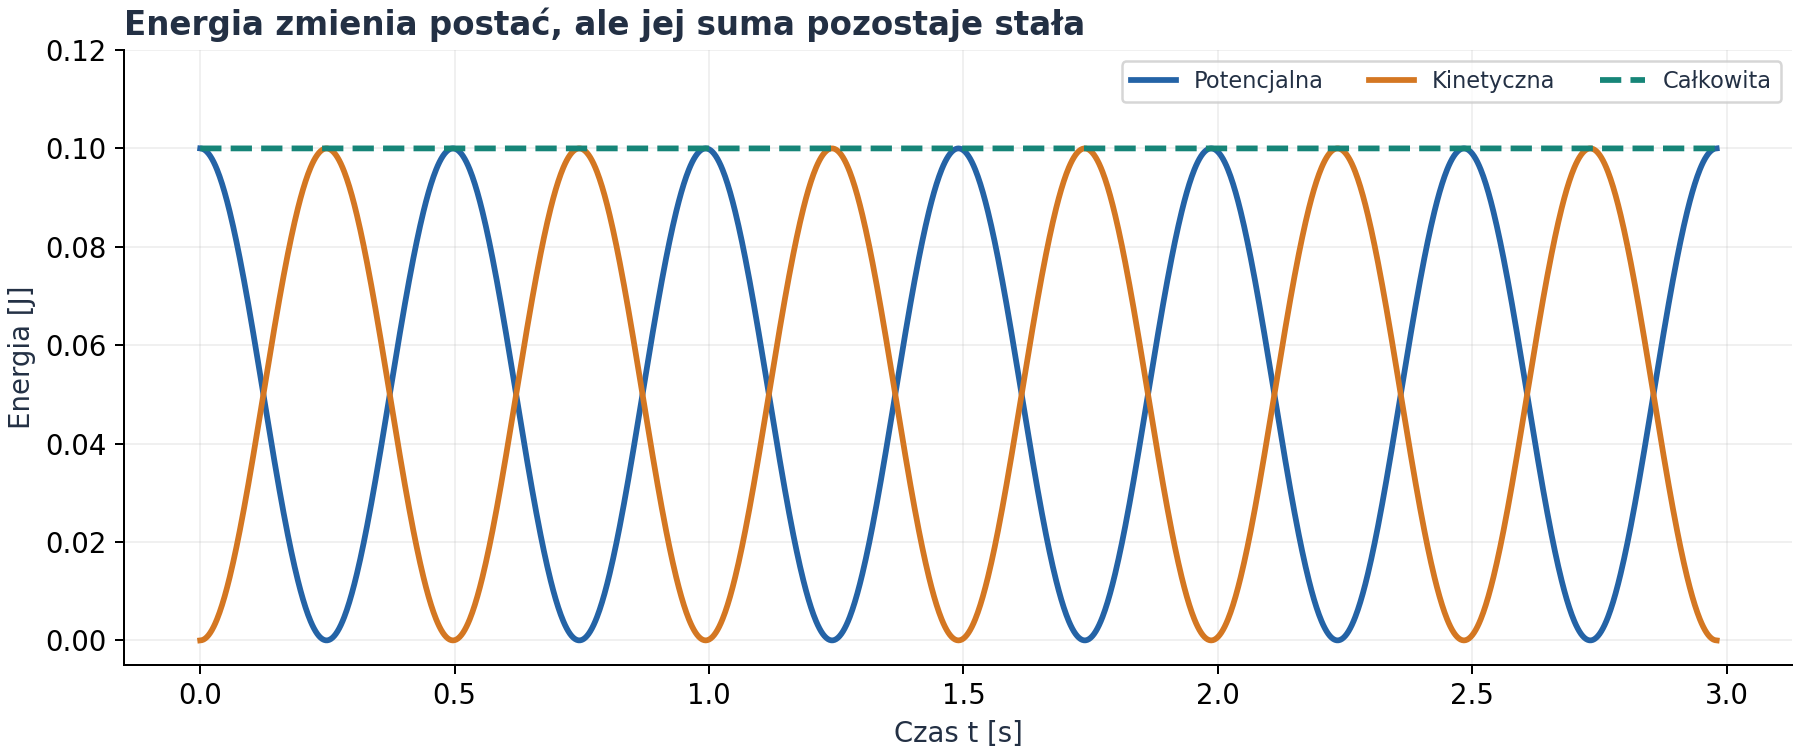
\includegraphics[width=\linewidth]{energia.png}
      \par\scriptsize Wykres modelowy: \texttt{pages/examples/01\_markdown}.
    \end{column}
  \end{columns}
\end{frame}

\section{Opory i wymuszenie}
\begin{frame}
  \frametitle{Tłumienie}
  Dla oporu lepkiego $-b\dot x$:
  \begin{equation*}
    m\ddot x+b\dot x+kx=0.
  \end{equation*}
  \begin{alertblock}{Uwaga}
    Przy $b>0$ energia mechaniczna maleje:
    $\dot E=-b\dot x^2\leq 0$.
  \end{alertblock}
\end{frame}

\begin{frame}
  \frametitle{Wymuszenie okresowe}
  \begin{equation*}
    m\ddot x+b\dot x+kx=F_0\cos(\Omega t).
  \end{equation*}
  Amplituda stanu ustalonego:
  \begin{equation*}
    A(\Omega)=
    \frac{F_0}{\sqrt{(k-m\Omega^2)^2+(b\Omega)^2}}.
  \end{equation*}
  \begin{itemize}
    \item Dla małego tłumienia maksimum leży blisko $\omega_0$.
    \item Tłumienie ogranicza wysokość maksimum.
  \end{itemize}
\end{frame}

\begin{frame}
  \frametitle{Dwie perspektywy}
  \begin{columns}[T]
    \begin{column}{.47\textwidth}
      \begin{block}{W czasie}
        Obserwujemy położenie $x(t)$ i okres
        $T=2\pi/\omega_0$.
      \end{block}
    \end{column}
    \begin{column}{.47\textwidth}
      \begin{exampleblock}{W przestrzeni fazowej}
        Stan określa para $(x,\dot x)$.
        Bez strat tor jest elipsą.
      \end{exampleblock}
    \end{column}
  \end{columns}
\end{frame}

\section{Wnioski}
\begin{frame}
  \frametitle{Najważniejsze wnioski}
  \begin{enumerate}
    \item Częstość własna zależy od $k/m$.
    \item W modelu idealnym energia jest zachowana.
    \item Opór odbiera energię, a wymuszenie może ją dostarczać.
  \end{enumerate}
  \medskip
  \centering\large $m\ddot x+b\dot x+kx=F_0\cos(\Omega t)$
\end{frame}
\end{document}
